\documentclass{beamer}
\title{Fooling Conv Nets}
\author{Shah Rukh Qasim\\
	Abdul Muiz Ahmed\\
	Tooba Imtiaz\\
	Muhammad Azeem Sabir\\
	Moeez Aziz\\
	Ahmed Alam
	}

\subtitle{Adding invisible noise}
\date{January 09, 2018}
%\addtobeamertemplate{navigation symbols}{}{%
%	\usebeamerfont{footline}%
%	\usebeamercolor[fg]{footline}%
%	\hspace{1em}%
%	\insertframenumber/\inserttotalframenumber
%}
\usepackage{graphicx}
\usepackage{algorithm}% http://ctan.org/pkg/algorithms
\usepackage{algpseudocode}

%\usetheme{Copenhagen}

\usetheme{CambridgeUS}

\begin{document}
	\section{Introduction}
	\subsection{Title}
	\frame{
		\titlepage
	}
	
	\section{AlexNet}
	\subsection{Intro}	
	\frame{
		\frametitle{Intro to the network}
		\begin{itemize}
			\item Krizhevsky et al. (AlexNet) \cite{krizhevsky2012imagenet}
			\item Presented in 2012
			\item Currently has 18,400+ citations
		\end{itemize} 
	}
	
	\subsection{I/O}	
	\frame{
		\frametitle{I/O}
		\begin{itemize}
			\item Input image is 3 channel 224x224
			\item There are many conv layers and 2 dense layers
			\item Trained on 1000 classes of image-net
		\end{itemize}
		
		\begin{center}
			\scalebox{1} {
				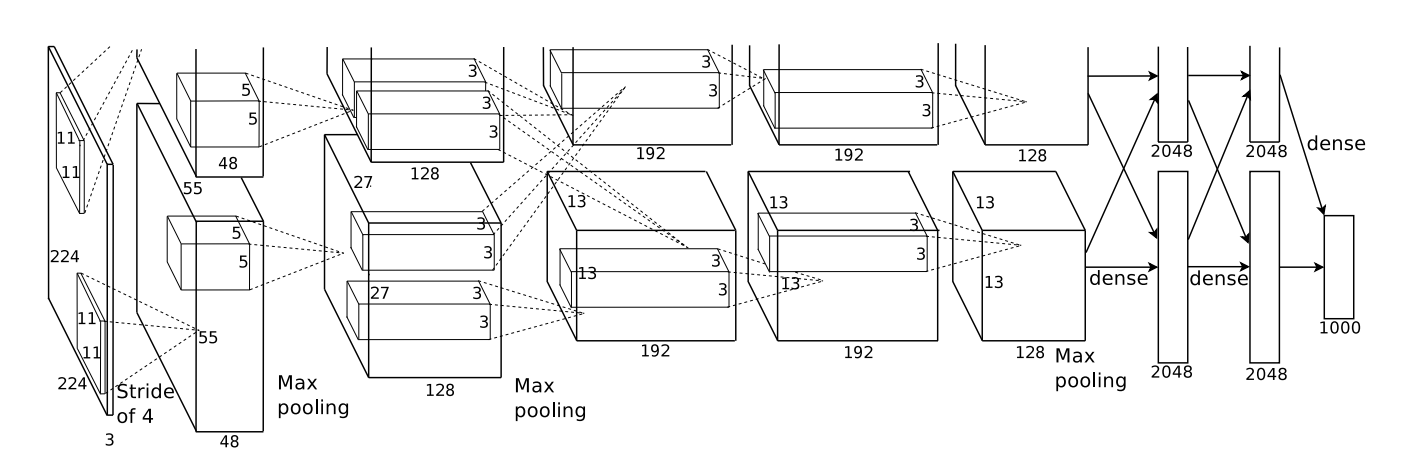
\includegraphics[height=3.3cm]{tex_images/01.png}
			}
		\end{center}
	}
	
	
	\subsection{Input Normalization}
	\frame{
		\frametitle{Input Normalization}
		\begin{itemize}
			\item Input image is normalized using z-transform
			\item z-transform is applied separately on different channels
			\item For dataset, $\mu = 0, \sigma = 1$ across different channels
		\end{itemize}
	}
	
	\subsection{Getting probabilities}
	\frame{
		\frametitle{Getting probabilities}
		\begin{itemize}
			\item Softmax is applied on last layer to get probability score
			\item $\Sigma x_i = 1$
			\item We pick the class with maximum probability score
			\item Softmax cross-entropy with logits is used during training
			\item We don't need to take softmax to pick maximum
		\end{itemize}
	}
	
	\section{Fooling}
	\subsection{Loss function}
	\frame{
		\frametitle{Loss function}
		\begin{itemize}
			\item Loss to fool the conv-net:\\
			\begin{align*}
				L = 1 - p_f
			\end{align*}
			\item f is the class to change the prediction to
			\item $p_k$ for any value of $k$ will not go above 1 guaranteed by softmax
		\end{itemize}
	}
	
	\subsection{Adding noise}
	\frame{
		\frametitle{Adding noise}
		\begin{itemize}
			\item Add noise to each channel
			\item The noise is random uniform initialized between 0 and 0.01
			\item This noise is very small to show any visible output
		\end{itemize}
	}
	
	\subsection{Optimizing noise}
	\frame{
		\frametitle{Optimizing noise}
		\begin{itemize}
			\item Apply descent on noise to minimize the loss function 
			\item On each pixel value
			\begin{align*}
			p'_{ij}&=p_{ij}+n_{ij}\\
			 \text{where}~p_{ij} &= \text{Pixel at location (i,j)} \\
			 n_{ij} &= \text{Noise at location (i,j)} \\
			 p'_{ij} &= \text{Modified pixel at location (i,j)}
			\end{align*}
			\item Subject to restraints
			\begin{align*}
			-c\textless &n_{ij}\textless c\\
			0\textless &p'_{ij}\textless 255\\
			\text{where}~c &= \text{Noise value clamp}
			\end{align*}
		\end{itemize}
	}
	
	\subsection{Loss reduction}
	\frame{
		\frametitle{Loss reduction}
		\begin{itemize}
			\item Adam optimizer \cite{kingma2014adam} is used for optimizing noise
			\begin{center}
				\scalebox{1} {
					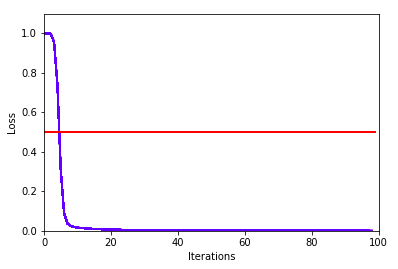
\includegraphics[height=3.5cm]{tex_images/02.png}
				}
			\end{center}
			\item The loss is easily converged in \textless 100 iterations
		\end{itemize}
	}
	
	\section{Conclusion}
	\subsection{Conclusion}
	\frame{
		\frametitle{Technologies used}
		\begin{itemize}
			\item Python 3.5 is used
			\item Pytorch \cite{paszke2017automatic} is used as differentiation engine
			\item Pillow is used for image loading
			\item Matplotlib is used for plots and image display
		\end{itemize}
	}
	
	\frame{
		\frametitle{Conclusion}
		\begin{itemize}
			\item The code is all public
			 \href{url}{https://github.com/shahrukhqasim/FoolingConvNets}
			\item With instructions on how to run
			\item Demo
		\end{itemize}
	}
	
	
	\section{References}
 	\subsection{References}
 	\frame%[allowframebreaks]
 	{
 		\frametitle{References}
 		\bibliography{present} 
 		\bibliographystyle{ieeetr}
 	} 	
\end{document}


